\chapter{Architecture}
Describe the different parts of your program suite in detail.
\\\\
kort inledning till kapitlet. vad har vi gjort i projektet?\\
trattigt namn, borde kanske ändras. ska innehålla typ metod - alltså vad har vi gjort?

\section{Finished work}
Running modules
What does your running code do? what is the output?

\subsection{Naive Bayes}

Naive Bayes was implemented using the prior probabilities $P(x_i\vert c)$ used in the Naive Bayes model $P(c\vert\mathbf{x})$, defined previously in Equation \ref{eq:naivebayes_model}. These were interpreted as the individual probabilities of each word $w$ from a vocabulary $\mathbf{V}$ occurring in class $c$, by exchanging $\left\{x_i : 1 \le i \le D\right\}$ for $\left\{w_i \in \mathbf{V}\right\}$ when using the model.
\\\\
The implementation of $P(w_i\vert c)$ follows the maximum likelihood estimate of relative frequency as follows:
\begin{align}
P(w_i\vert c) =
\frac
	{
		\sum_{d \in \mathbf{D}} F_{w_i}^{(d)}
	}
	{
		\sum_{w_j' \in \mathbf{V}} \sum_{d \in \mathbf{D}}  F_{w_j'}^{(d)}
	},
\end{align}
where $F_w^{(d)}$ defines the relative word frequency in document $d$ from corpus $\mathbf{D}$, implemented with the following two options to be compared:
\begin{description}
  \item[Binary frequency:] Boolean $\in \left\{0,1\right\}$ if word $w$ occurs in document $d$,
  \item[Tf-idf:] $\frac{\texttt{Normalized term frequency}}{\texttt{Document frequency}} \in \left[0, \log \left\vert \mathbf{D}\right\vert\right]$.
\end{description}
A caveat with this procedure is that since both of these options allow for $F_{w_i}^{(d)}$ to be zero, the product in the Naive Bayes model (\ref{eq:naivebayes_model}) for $P(c\vert d)$ vanishes for all combinations of classes $c$ and documents $d$ for which $d$ includes a word $w_i$ that never occurs in the given class. To assure nonzero prior probabilities Laplace smoothing was used, which adds one to each count as follows \citep{nb_ref}. 

\begin{align}
P(w_i\vert c) =
\frac
	{
		1 + \sum_{d \in \mathbf{D}} F_{w_i}^{(d)}
	}
	{
		\left\vert\mathbf{V}\right\vert + \sum_{w_j' \in \mathbf{V}} \sum_{d \in \mathbf{D}} F_{w_j'}^{(d)}
	},
\end{align}
The parameter $P(c)$ is implemented as
\begin{align}
P(c) = \frac{\left\vert\mathbf{D}_c\right\vert}{\left\vert\mathbf{D}\right\vert}
\end{align}
where $\left\vert\mathbf{D}_c\right\vert$ is the number of documents with class $c$. The training algorithm is shown in Algorithm \ref{algorithm:naive_bayes_training}.\\\\\\\\\\\\\\\\\\\\\\\\\\\\\\\\\\\\\\

\begin{algorithm}[h]
 \SetAlgoLined
 
 \KwData{\textit{Word Tf-idf-values} $\left\{F_{w_i}^{(d)} : d \in \mathbf{D}, 1 \le i \le \left\vert\mathbf{V}\right\vert\right\}$;
 		 \textit{Training classes} $\left\{c_d : d \in \mathbf{D}, c \in \mathbf{C}\right\}$; \textit{Using Tf-idf boolean} \texttt{use\_tfidf}}
 \KwResult{$P(c), P(w\vert c)$}
  \For{$i=1$ \KwTo $\left\vert\mathbf{C}\right\vert$}
  {
  	class $\leftarrow c_i$\\
  	P(class) = $\frac{\left\vert\mathbf{D}_c\right\vert}{\left\vert\mathbf{D}\right\vert}$
  }
 \ForEach{$d \in \mathbf{D}$}
 {
	class $\leftarrow c_d$\\
	\For{$i=1$ \KwTo $\left\vert\mathbf{V}\right\vert$}
	{
		word $\leftarrow w_i$ \\
		\uIf{\texttt{use\_tfidf}}
		{
			$P($word$\vert$class$)$ += $T_{w_i}^{(d)}$
		}
		\Else
		{
			$P($word$\vert$class$)$ += $1$
		}
	}
 }
 Normalize($\left\{P(w\vert c) : w \in \mathbf{V}, c \in \mathbf{C}\right\}$)\\
 \Return $\left\{P(c), c \in \mathbf{C}\right\}, \left\{P(w\vert c) : w \in \mathbf{V}, c \in \mathbf{C}\right\}$
 \caption{Multinomial Naive Bayes training algorithm}
 \label{algorithm:naive_bayes_training}
\end{algorithm}


\subsection{K-Nearest Neighbour (KNN) algorithm}
The KNN algorithm was implemented by interpreting each feature, or in this case
every document, as a dimension and feature values corresponds to the term
occurrence frequencies. Calculations of the nearest neighbours were
implemented in a non deterministic way. This because of that a point $x$ in a plane
may have neighbours with the property that they have equal distances to
$x$. If this is the case a nearest neighbour is chosen at random. Several choices
for $k$ were tested in different runs of the algorithm to find the best $k$ for
the classification. The algorithm was implemented to be able to classify both
different classes (music , software, etc.) and sentimental classification
(positive, negative). Figure \ref{fig:KNNplot} shows the misclassification done by the
algorithm for both different $k$ and different sizes of the feature sets. The plot was generate with training set size 2000 and test set size 100 for unigrams. Note that the result might look different for other training set sizes. We used the best $k$ from this plot which is full training set size.
\begin{figure}[h!]
\centering
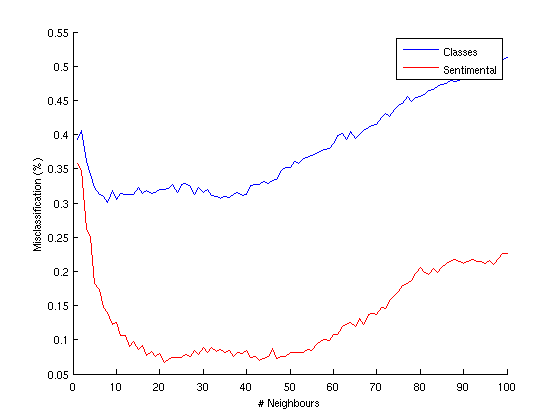
\includegraphics[scale=0.6]{../Plottar/knn_2000words_testdata100_unigram}
\caption{Plot showing results from the KNN classifier}
\label{fig:KNNplot}
\end{figure}\\
Figure \ref{fig:KNNplot} shows that KNN has best performance with parameter $K = 20$ for sentimental and $K = 10$ for classes.

%\begin{comment}
%The pseudocode below described the implemented matlab code.

%\begin{algorithm}[H]
% \SetKwData{Left}{left}\SetKwData{This}{this}\SetKwData{Up}{up}
% \SetKwFunction{Union}{Union}\SetKwFunction{FindCompress}{FindCompress}
% \SetKwInOut{Input}{input}\SetKwInOut{Output}{output}
% \Input{A data set X, A vector of labels Y,Number of nearest neigbour k,A feature vector x}
% \Output{A classification index}
% $\forall$ documents in data calculate the distances $D$ to $x$\;
% SDI = Sort the vector D and get the indexes in D \;
% S = A zero vector of size equal to the number of labels \;
%
% \For{i $\in$ \{1 \ldots k\}}{
%  read current\;
%  \eIf{understand}{
%   go to next section\;
%   current section becomes this one\;
%   }{
%   go back to the beginning of current section\;
%  }
% }
% \caption{How to write algorithms}
%\end{algorithm}

\subsection{Support Vector Machine (SVM)}
We choose to use the matlab library $svmtrain$ \citep{svmtrain_ref} from the Statistics toolbox. Svmtrain was used hard-margined and configured such that when it didn't converge we set the classification to all zero, which would represent $100\%$ misclassification. \\
\begin{algorithm}[H]
\label{algorithm:SVM}
\SetAlgoLined
\KwData{Xtraining: The data to train, Ytraining: labels of data to train \\ Xtest: The data to test}
\KwResult{Vector containing the classified labels}
\SetKwData{Try}{try}
\SetKwData{Catch}{catch}
\SetKwData{End}{end}
\SetKwIF{Try}{Elseif}{Catch}{try}{:}{else if}{catch:}{}

Set max iterations 150000 \\
\Try{}{
svm$\_$model = $svmtrain(Xtraining, Ytraining, linear)$ \\
classifications = $svmclassify(svm\_model, Xtest)'$
}\Catch{$classifications = zeros( Xtest)$}{}{end}
 \caption{SVM using svmtrain}
\end{algorithm}



\subsection{The Perceptron algorithm}
The Perceptron algorithm works as follows:
The output, $w$, from the algorithm is a weight vector with the same size as $y$. If the classification for a $x$ in the training set is equal to $y$, the weight is unchanged.
If $y$ is 1 and the classification -1, then $w$ is increased. If $y$ is -1 and the classification 1, then $w$ is decreased. \citep{perceptron_ai}
\begin{algorithm}[h!]
\label{algorithm:perceptron}
 \SetAlgoLined
 \KwData{data}
 \KwResult{weight vector $w$}
 Initialize weight vector $w$ to all zeros\;
 $N \leftarrow$ number of iterations through training set\;
 \For{1 $\rightarrow$ N}{
   \ForAll{x, y in the training set}{
    $guess \leftarrow classify(x)$ using our current $w$\;
    \If{y is not equal to guess}{
     $w \leftarrow w + f(x, y) - f(x, guess)$\;
     }
   }
 }
 \caption{Perceptron}
\end{algorithm}
The Averaged Perceptron works in the same way except that it returns the average weight vector instead of the final.
This averaged vector is built incrementally by updating it while we build the usual weight vector. The pseudo code almost the same as for the usual perceptron.
\begin{algorithm}[h!]
\label{algorithm:perceptron}
 \SetAlgoLined
 \KwData{data}
 \KwResult{weight vector $w$}
 Initialize weight vector $w$ and the average weight vector $wa$ to all zeros\;
 Initialize the counter $c$ to 0\;
 $N \leftarrow$ number of iterations through training set\;
 \For{1 $\rightarrow$ N}{
   \ForAll{x, y in the training set}{
    $guess \leftarrow classify(x)$ using our current $w$\;
    \If{y is not equal to guess}{
     $w \leftarrow w + f(x, y) - f(x, guess)$\;
     $average\_weight \leftarrow (N\cdot T - c) / (N\cdot T)$
     $wa \leftarrow wa + average\_weight \cdot (f(x, y) - f(x, guess))$
     }
     Increase the counter c
   }
 }
 \caption{Averaged Perceptron}
\end{algorithm}
In both of the Perceptron algorithms, the algorithm makes a number of iterations. To decide how many iterations that must be done to get a fair result the misclassifications and the number of iterations were plotted, which is shown in Figure~\ref{fig:number_iterations}. The algorithms uses input data of 2000 words (unigram) and 10-fold crossvalidaion. As seen in the plot, both the algorithms converge after around 15 iterations for both sentimental classification and text categorization.
\begin{figure}[h!]
\centering
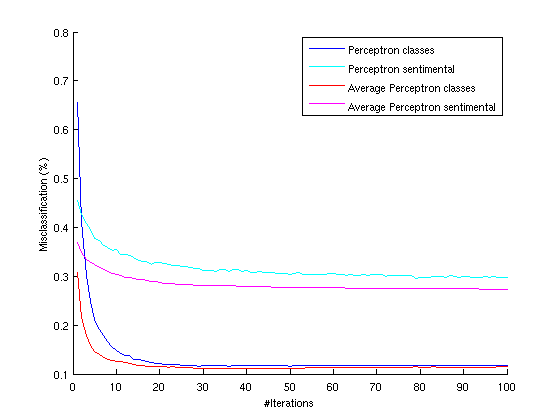
\includegraphics[scale = 0.8]{fig/perceptron_2000words_unigram_10foldcv_classes-high_sentimental-low.png}
\caption{Plot over misclassifications for different \#iterations}
\label{fig:number_iterations}
\end{figure}\\
Since the Perceptron algorithms are 0/1 classifiers there is some difficulties with classifying the data as classes. This was solved by for all data and all classes classify the data as belonging to this class or not. Finally the new document is classified as the class it belongs to most.

